%%!Mode:: "Tex:UTF-8"
\documentclass[notypeinfo,xelatex]{CASthesis}
% 可选参数:
% notypeinfo 取消扉页的LaTeX版本信息
%
% 下面三个选一个:
% dvipdfm 使用 dvipdfm(x) 生成最终的 PDF 文档 (缺省设置)
% dvips 使用 dvips 生成最终的 PS 文档
% pdftex 使用 pdfLaTeX 生成最终的 PDF 文档

% 设置图形文件的搜索路径
\graphicspath{{figures/}}

% 取消链接的颜色(黑白打印时)
\hypersetup{colorlinks=false}

% 小节标题靠左对齐
%\CTEXsetup[format+={\flushleft}]{section}
%\titleformat{\chapter}[display]{}{\songti}{1em}{}
\CTEXsetup[format+={\songti}]{section}
\CTEXsetup[format+={\songti}]{subsection}
%\usepackage{titletoc}
\usepackage{multicol}
%\renewcommand{\thechapter}{}
\CTEXsetup[number={\arabic{chapter}}]{chapter}

%\usepackage[title]{tocloft}
%\renewcommand{\cfttoctitlefont}{\normalfont\MakeUppercase}

%\renewcommand\cftchapfont{\songti\zihao{4}}
%\renewcommand\cftsecfont{\songti\zihao{4}}
%
%\renewcommand\cftchappagefont{\songti\zihao{4}}
%\renewcommand\cftsecpagefont{\songti\zihao{4}}

\begin{document}


%%%%%%%%%%%%%%%%%%%%%%%%%%%%%%
%% 封面部分
%%%%%%%%%%%%%%%%%%%%%%%%%%%%%%

  % 中文封面内容
  \classification{O212}
  \confidential{公开}
  \UDC{519.2}
  \serialnumber{}

  \title{随机环境中带分散自适应牵制控制的复杂网络簇同步问题}
  \englishtitle{English title}
\titlepageone{随机环境中带分散自适应牵制}
\titlepagetwo{控制的复杂网络簇同步问题}
  \author{叶丹凤}
  \advisor{董海玲~副教授}
  \advisorinstitute{}
  \subject{理学}
  \major{统计学}
  \submitdate{2016年4月}
  \defenddate{2016年4月}
  \institute{数学与统计学院}
  \school{深圳大学}
  \schoolid{10590}
  \degree{硕士}
  \chairman{}

  % 英文封面内容


  % 封面
  \maketitle

  % 英文封面
 % \makeenglishtitle

\declare
%%%%%%%%%%%%%%%%%%%%%%%%%%%%%%
%% 前言部分
%%%%%%%%%%%%%%%%%%%%%%%%%%%%%%
\frontmatter

  % 摘要
  %%!Mode:: "Tex:UTF-8"
\begin{abstract}
\vspace{2ex}
复杂网络在各个学科和领域都有着普遍的应用, 同步又是复杂网络一种具有代表性的群体行为. 最近几年, 复杂网络同步问题的研究吸引了越来越多研究者的关注, 研究者们在各类同步问题上取得了较大的进展. 然而, 大多数同步结果都是建立在连续通讯模式下, 即网络节点间的信息状态实时更新并且实时传递. 这不仅浪费通讯带宽而且降低网络抗干扰能力, 从而使得网络不稳定. 因此考虑离散通讯模式的控制策略有着更加实际的意义.

本学位论文主要讨论在随机环境下, 如何构造合适的事件激发规则并结合相应的控制方法来实现马氏耦合复杂网络的同步. 主要工作包括以下几个方面:

首先介绍了复杂网络背景和同步研究现状以及同步的相关定义、随机过程理论相关基础知识. 同时也介绍了证明定理过程中所用的引理及符号说明.

其次讨论非线性耦合拓扑与随机发生的耦合以及随机耦合强度并存的复杂网络均方指数同步问题. 引进Bernoulli随机变量和正态随机变量来刻画随机发生耦合和随机耦合强度. 为了降低网络间通讯的频率以及控制器的更新频率, 分别在连续监控和离散监控两种情形下, 设计两种基于不同误差上界的分散式事件激发规则. 采取分散式事件激发采样策略和牵制控制相结合的控制方法, 对网络几个关键节点实行牵制控制. 根据Lyapunov 稳定性理论、随机过程理以及Gronwall-Bellman不等式推导复杂网络能够实现均方指数同步的充分条件. 通过经典蔡氏电路数值仿真不仅证实给出的判据能够保证网络达到同步, 同时在数值上比较四种不同激发规则在同步速度和激发频率上的差异.

接着研究带有时滞与部分未知转移率的马氏耦合复杂网络同步问题. 网络节点之间的拓扑关系不仅存在模式切换, 而且模式间切换概率是部分未知的. 另外, 节点动力学受到时滞的影响. 除此之外, 还考虑了动态调整的同步目标. 利用集中式的事件激发采样策略, 对网络的节点以概率$p$进行随机控制来促使网络达到同步. 通过构造新的随机Lyapunov-Krasovskii函数, 基于随机过程理论、Lyapunov 稳定性理论、以及Halanay不等式得出同步的充分条件. 最后给出事件激发间隔下界保证Zeno现象在事件激发采样控制策略下不会发生. 数值模拟的结果显示, 事件激发采样控制策略能够促使网络快速达到同步, 并且两事件激发时刻具有明显的间隔.

最后, 在转移概率部分未知的基础上, 进一步研究带有噪声干扰的复杂网络同步问题. 不同于自身节点动力学的噪声, 本文考虑的是节点之间的信号传输过程遭受的噪声, 其噪声由布朗运动产生. 根据测量误差和同步误差, 分别构造出集中式和分散式事件激发规则. 利用稳定性理论和伊藤—德布林公式, 推导出同步条件. 数值例子验证了理论结果的有效性.
\vspace{2ex}

\keywords{同步; 事件激发策略; 马氏链; 部分转移率未知; 布朗运动}

\end{abstract}

\begin{englishabstract}
\vspace{2ex}
Complex networks have applied widely in the domain of science, and synchronization is a typical cluster behavior of complex networks. In recent years, more and more researchers have been attracted by the problem of synchronization of complex networks, and major result has been established. However, almost all of these results are built upon the assumption that the communication of nodes are a continue mode.  Namely, the information between the nodes in networks update and transmit immediately, which would not only lead to wasting of communication bandwidth, but also reduce anti-interference ability. So the discrete mode communication control strategy are more practical significance.

This paper mainly discuss how to construct a suitable event-triggered rule and corresponding control method to achieve synchronization of complex networks with Markov switching in random environment. The main work includes the following aspects:

First of all, we introduce the background of complex networks and research status about synchronization and corresponding definitions, basic knowledge of random process theory, lemma and some symbols needed in this paper.

Secondly, the mean square exponential synchronization issues of complex networks with Markov switching nonlinear and randomly occurring coupling topology and random coupling strength are studied. Bernoulli random variable and normal random variable are introduced to depict random occurring coupling and random coupling strength. In order to reduce the frequency of communication between the network and the update of the controller, Two different decentralized event-triggered rules base on synchronization error upper bound and exponential upper bound are proposed in the continuous monitoring and discrete monitoring. The key nodes are pinned to prompt the networks realizing synchronization by using control method with decentralized event-triggered sample strategy and pinning control. According to Lyapunov stability theory, the stochastic process theory and Gronwall-Bellman inequality, the sufficient condition of mean square exponential synchronization are derived. In the numerical example part, it is not only confirm the synchronization condition is valid vote, but also compare the differences about four different rules in the synchronous speed and triggered frequency.

Next, we study exponential synchronization problems for an array of Markovian jump delayed complex networks with partially unknown transition rates. In the networks model, the topological relationship between nodes not only switch in limited mode, but also the switching probability are partially unknown, and the node dynamic behavior is time-delay. In addition, the synchronization trajectory is dynamic. To impel the array complex networks to achieve exponential synchronization, a new randomly occurring event-triggered control strategy is proposed with the probability $p$ base on centralized event-triggered sample strategy. By constructing a novel stochastic Lyapunov-Krasovskii function, some exponential synchronization criteria are obtained in terms of LMIs and famous Halanay inequality. Furthermore, we obtain a positive lower bound of the event intervals which can exclude the Zeno behaviors in event-triggered sample strategy. Numerical simulation show that the  event-triggered sample control strategy can achieve synchronization rapidly and there has obvious gap between two event-triggered moment.

Finally, the issue of synchronization of complex networks perturbed by stochastic noise are further researched base on partially unknown transition rates. The stochastic noise appear in the signal transmission process between the nodes rather than the node's dynamics which is produced by the Brownian movement. According to the measurement error and synchronization error, the centralized and decentralized event-triggered rules are provided. By using stability theory and inequalities of stochastic integral, some exponential synchronization criteria are obtained. A simulation example is provided to demonstrate the effectiveness of the theoretical results.
\vspace{2ex}

\englishkeywords{Synchronization; Event-Triggered Strategy; Markov Chain; Partially Unknown Transition Rates; Brownian Movement}
\end{englishabstract}


  % 目录




\tableofcontents

  % 表格目录
  %\listoftables
  % 插图目录
  %\listoffigures


%%%%%%%%%%%%%%%%%%%%%%%%%%%%%%
%% 正文部分
%%%%%%%%%%%%%%%%%%%%%%%%%%%%%%
\mainmatter

  %!Mode:: "Tex:UTF-8"
\chapter{引言}\label{chap:introduction}


\section{复杂网络的研究背景及意义}

随着人类的进步和社会的发展, 人与人之间、人与自然界之间以及自然与自然之间形成各种千姿百态、形形色色的复杂网络系统, 例如社交关系系统、电力系统、航空系统、万维网、食物链、疾病传播系统、蛋白质相互作用系统等等. 人们为了研究这些网络系统的特征和性质, 抛开系统的物理和社会含义, 把系统中互异的元素称之为节点(node), 把元素之间的关系用连边(edge) 来表示, 于是物理网络系统都可以抽象为由节点和连边组成的复杂网络模型. 例如, 在社会关系系统中, 可以把每一个人看做网络的节点, 如果两个人之间相互认识, 那么就用连边表示; 在航空系统网络中, 我们可以把各个城市看做网络的节点, 若城市之间存在航线, 就用连边来表示. 由此可见, 任何一个复杂的网络系统都可以将其抽象成为具有节点和连边的网络结构. 这种从具体网络模型上升到抽象网络模型的思想给研究者探索网络内部结构的复杂性提供了一种新思路.

这种将真实网络中的实体与实体之间的关联抽象化成为节点和连边所组成的复杂网络的思想是源于$18$世纪$30$年代著名数学家Eular论证哥七桥问题. Eular首次将真实存在的物理关系抽象为节点与连边, 从而开创图论学科, 使网络研究最终独立成为一门学科. 从此掀起了科学家们对网络科学理论的研究热潮. 早些年, 研究者们研究的网络模型都是具有某种特殊结构的网络, 也就是说网络中的节点与节点关系遵循一定的规律, 这种网络称为规则网络. 主要的规则网络有完全连接网络、最近邻连接网络、星形网络、Lattice网络、Layers网络等. 但是对于大规模网络而言, 它的复杂程度并不是都能采用规则网络来表征.

1960年前后, 两位杰出的数学大师Erdös与Rényi创立了著名的随机图理论, 从而为随机网络(ER Network)的发展奠定了理论基础. 随机网络与规则网络最大的不同点在于网络节点间的关系不再是确定的, 而是以一定的概率随机连接的. 由于复杂网络节点之间的关系是受到随机变量的控制, 从而使得网络耦合拓扑空间变得更为复杂, 并且在数学性质上与规则网络也存在质的不同, 很多规则网络的性质在随机网络中不在成立. Erdös和Rényi两人在研究时发现, 随机网络的重要特征和性质都是随着节点数量的扩大而突出出现的.

\begin{figure}[htb]
\begin{minipage}[t]{0.48\linewidth}
\centering
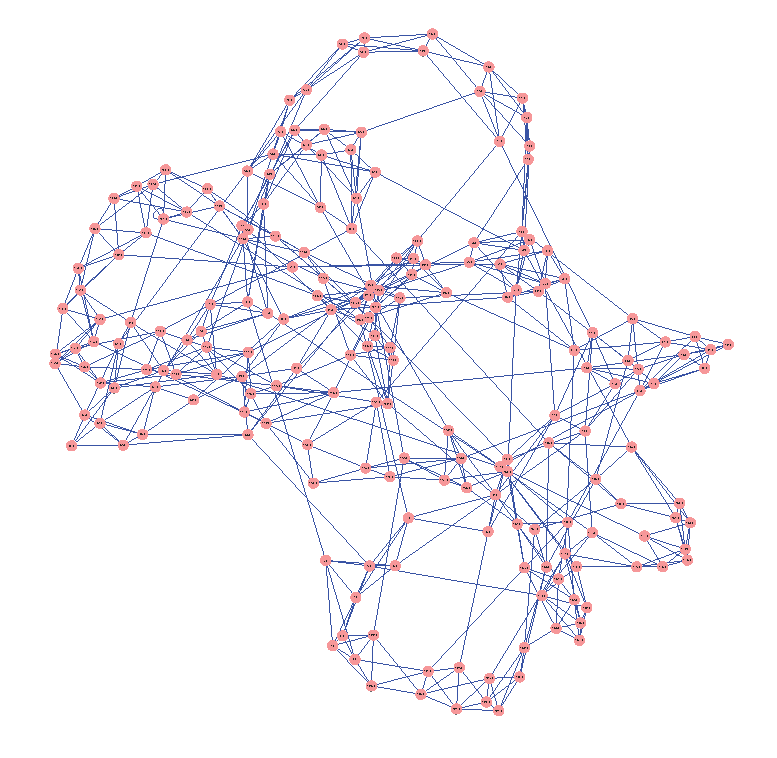
\includegraphics[width=2.5in]{introduction/wattsstrogatz.eps}
\caption{小世界网络.}\label{smallworld}
\end{minipage}~~
\begin{minipage}[t]{0.48\linewidth}
\centering
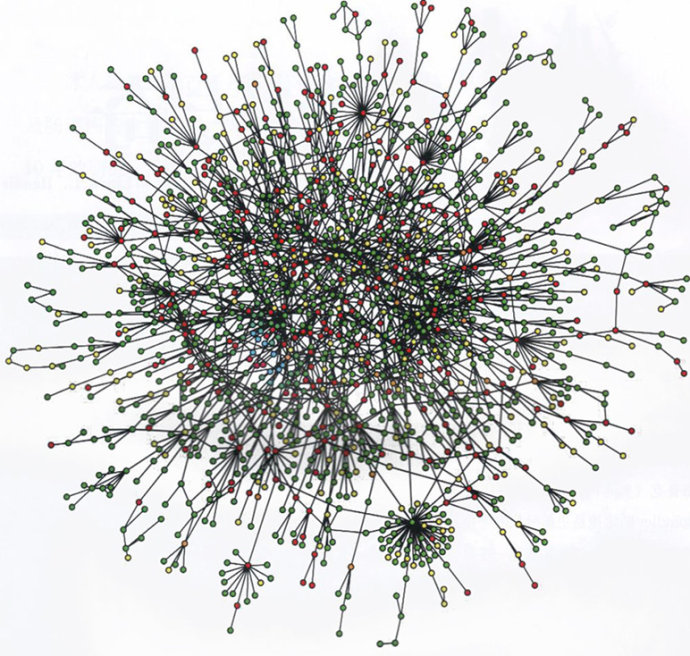
\includegraphics[width=2.5in]{introduction/scale.png}
\caption{无标度网络.}\label{scalefree}
\end{minipage}
\end{figure}

20世纪末, 科学家们发现, 很多网络都具有高度的集群性、不均衡的度分布以及中心节点结构. 这类结构的网络恰好是介于规则网络和随机网络之间, 但是它的统计特征与规则网络和随机网络截然不同. 国际上出现两项具有里程碑意义工作: Watts 和Strogatz在1998年定义了一种新型网络—小世界网络\upcite{2}(如图 \ref{smallworld}). 小世界网络介于规则网络和随机网络之间, 它是在规则网络的基础上以一定的概率断开连边后在重新随机连接其他的节点所形成的网络. 当切断连边的概率取$0$、$1$ 两个极端值的时候, 此时就变成规则网络和随机网络(如\autoref{SWN}). 生活中的很多网络都表现出小世界特性, 例如蛋白质分子相互作用网、手机通讯网络、科学引文网以及社会关系网等. 小世界网络的提出, 进一步证实了“六度分离”假说.

%在小世界网络出现之前, 人们认为网络分为完全规则网和完全随机网, 这两类网络具有各自的特征. 规则网络具有较大的特征路径长度, 聚类系数也较大, 而随机网络具有较小的特征路径长度, 但是聚类系数较小. 但现实中的网络如电网、交通网络、脑神经网络、社交网络、食物链等都表现出小世界特性, 即具有较高的聚类度和较小的特征路径长度. 也就是说小世界网络中大部份的节点彼此并不相连, 但绝大部份节点之间经过少数几步就可到达.
\begin{figure}[htb]
  \center
  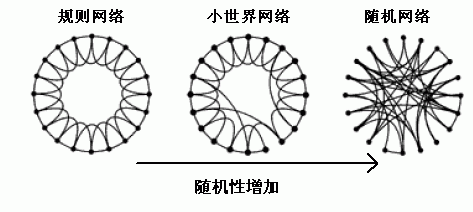
\includegraphics[width=3.3in]{introduction/smallnetwork.png}\\
  \caption{规则网络、小世界网络、随机网络之间的关系.}\label{SWN}
\end{figure}

一年后, Barabási等人于1999年在《科学》杂志上出了另外一种非均匀的网络模型——无标度网络\upcite{0}(如\autoref{scalefree}). 这类网络不仅拥有较大的聚类特性和较小的平均路径长度, 而且节点的度服从幂律分布. 许多复杂网络系统, 例如因特网路由关系网, 人力资源关系网等, 其网络中的大多数节点都是与某些特殊的节点有关联, 即网络中存在个别具有主要控制能力的节点. 这种网络节点间关系的不均匀性称为无标度网络的无标度性, 这种不均匀性是网络内在的一种性质.
复杂网络的“小世界”与“无标度”等统计特性的发现, 不仅丰富了网络内部结构的拓扑形式, 更进一步推动了研究者对复杂网络结构不断探索的热潮, 同时也加快了复杂网络理论在各个学科的研究进程\upcite{4,5,6,7,8,9,10}.

进入21世纪后, 小世界效应和无标度特性的提出使得复杂网络的理论研究踏上新台阶 , 并形成多学科交叉的理论成果. 近年来, 众多理论模型和分析方法如雨后春笋般涌现, 并且尝试利用复杂网络理论成果来解决各领域的实际问题. 目前主要研究工作分为: 一是研究网络内部耦合结构的变化以及统计性质, 例如网络系统的平均路径长度、聚集系数、度及度分布、谱性质、介数、小世界效应、无标度特性等特征; 二是研究复杂网络动力学行为, 包括鲁棒性、稳定性、一致性、以及同步问题等; 三是复杂网络在各个领域的应用, 包括生物医学、保密通信、图像处理、交通运输等领域\upcite{15,16,17}.


\section{复杂网络同步控制及其研究现状}
同步(synchronization)指的是两个或者两个以上性质相同或相似的动力系统通过系统节点之间的相互影响使得各个节点的动力学行为随着时间演变慢慢地趋于同一步调. 复杂网络的同步是一种群集行为. 自然界中同步现象数不胜数, 其中两个最为经典的同步现象是: 1665年, 荷兰物理学家、数学家惠更斯发现自家墙上的两个挂钟不论钟摆开始时如何摆动, 一段时间后, 两个摆钟的摆动频率完全相同, 摆动的方向恰好相反; 1680年, 荷兰旅行家肯普弗在旅行时注意到一个奇特的现象: 停留树枝上的萤火虫闪光的频率非常有规律, 几乎都是同时闪或者不闪. 除此之外, 生活中还存在各式各样的同步现象, 例如鱼群朝同一方向游动, 大雁群的一致飞行, 演唱会观众的拍手声等等.

1990年Pecora和Carroll\upcite{10}发现了一类混沌系统的同步现象, 由此开启了同步理论的研究新篇章. 目前已经出现了各种不同形式的同步模式:
有限时间同步\upcite{finitetimesyn}、固定时间同步\upcite{fixsyn}、完全同步\upcite{abssyn}、 簇同步\upcite{clusyn}、位相同步\upcite{phasyn}、指数同步\upcite{23}. 其中, 完全同步指的是只需要当时间趋于无穷时, 网络所有的节点之间的误差趋于零, 它是同步模式中最普遍的一种. 而指数同步是指误差以指数形式趋于零, 它是比完全同步具有更快同步速度的同步模式. 本文仅讨论这两种同步模式.

在近十多年里, 人们对各种复杂网络拓扑模型的同步问题进行了广泛地研究并积累了大量的研究成果\upcite{Karimi5,Multi6,Lu7,Liu8,Karimi10,Lu9,Turci11,Jin12,Turci13}. %2014 年Wang和Tang等人\upcite{p30,p31}对近十年来复杂网络的研究成果进行了概括总结, 并指出未来复杂网络研究的挑战.
但大多数的研究成果都是基于理想的假设: 网络所处的环境是保持不变的, 即网络的耦合结构、耦合强度是固定的, 且网络节点间的通讯不会受到其他外在因素的干扰. 然而, 在实际问题中, 这个假定很难被认为是合理的. 事实上, 在现实应用中, 网络系统的节点状态、耦合结构和耦合强度不可避免地遭受来自外部随机因素的干扰.
例如电力输送网会受到地震、火灾、雷击、输变电系统短路等不可预知因素的影响; 保密通讯会受到黑客的攻击等等.
因此考虑随机环境下的网络同步更加具有实际意义.
最近几年, 研究者们开始重视随机环境下复杂网络同步问题, 并且现在成为了一个较为活跃的研究方向. 随机环境下复杂网络同步问题研究的主题包括: 一是运用连续时间马尔可夫链来模拟耦合结构受随机环境影响而切换的变化过程\upcite{Li15,p10Markovian,p11Markovian,mm19,M20,M21,M22,M23,M24,M25,M17}; 二是引入随机变量来刻画耦合强度的随机性以及随机发生的耦合关系\upcite{X18,M19,randomcoupling1}; 三是通过布朗运动来模拟随机噪声对网络节点自身以及节点之间信号传输过程的干扰\upcite{Eventmultiagentnoises,p29,p30,p31,p32}. 尽管随机环境下复杂网络同步问题的研究取得较大的进展, 但还有许多问题亟待解决.
例如, 节点间状态信息的传输并非是简单的线性可观测形式, 而是通过非线性映射后的形式; 信息传输的有限速度和带宽引起网络节点自身动力学时滞的问题, 马尔可夫链转移率获取困难而引起的部分未知转移率的切换拓扑同步问题, 等等. 这些问题的解决能够更进一步完善复杂网络同步理论.

在现实生活中, 网络很难依靠自身节点之间的拓扑关联实现同步(自然同步)\upcite{phasyn,natsyn}. 这是由于网络内部节点庞大, 节点间的关联较为稀疏, 并且网络节点的关系会遭受到外部随机因素的干扰. 因此, 需要对网络施加外力, 即通过设置控制器来促使网络实现的同步.
目前, 很多控制策略被提出. 比较经典而且经济的控制策略是牵制控制\upcite{pin1,pin2,pin3}. 它只需要控制系统中极少数重要的节点, 然后通过节点的耦合关系将控制输入信号传送到其他的节点, 从而使得整个网络在控制节点的带领下达到同步状态. 相对于全局控制, 牵制控制具有可操作性强且节省控制成本的优势.
然而, 很多全局控制或者牵制控制的同步成果都是在连续通信模式下建立的, 这使得系统连续不断地更新自身信息状态和控制输入信号, 并且实时地向邻居节点发送当前状态信息. 显然, 这种模式会导致不必要的带宽和能源消耗, 加大了网络的通讯负荷, 并且降低了网络抗干扰能力.

随后, 研究者们提出了数据采样机制来降低节点间的通讯以及控制输入的更新频率, 数据采样机制主要有周期采样\upcite{period}以及事件激发采样. 根据周期选取的不同, 周期采样又分为固定周期采样、时变周期采样、以及随机周期采样. 相对于连续通信模式, 周期采样以可变频率进行采样并更新节点状态和控制项, 一定程度上节省了控制成本, 并且减少了节点间的通讯频率. 尽管周期采样模式能够减小能量的消耗和降低网络的通讯负荷, 但是该通讯模式对周期的选择较为敏感, 若周期过短会导致较大的计算负荷, 若周期过长会导致同步速度较慢. 除此之外, 网络不能够根据各个节点的状态自动地改变采样数据的频率. 不同于周期采样, 事件激发采样机制能够根据网络自身节点间的关系以及节点与同步目标之间的误差来决定采样时刻, 即系统能够根据自身的运行状况自适应地调整采样时间点, 事件激发采样机制正好弥补了周期采样在周期选择上的缺陷. 事件激发采样控制策略被广泛应用于多主体系统一致性控制问题\upcite{Eventmultiagentnoises,eventmult2,eventmult3,eventmult4,eventmult5,eventmult6,eventmult7,eventmult8,eventmult9}, 最近有研究者开始关注事件激发采样控制策略在复杂网络同步问题的研究, 并取得了一些进展性工作\upcite{eventsyn1,eventsyn2,eventsyn3,eventsyn4,eventsyn5,eventsyn6,eventsyn7}. 事件激发采样模式的主要思想是: 当系统节点与同步目标之间的偏差大于给定的阈值时, 此时事件被触发, 节点就更新自身的状态和控制项, 并向邻居节点传递信息. 换句话说, 网络节点的信息更新和信号的传输只发生在事件激发时刻. 事件激发采样控制模式最大的特点是网络根据节点自身的状态按照需要进行更新和传递数据信号, 从而能够极大减少通信的频率, 节省能量. 正如K. {\AA}ström\upcite{eventsyn8} 和B. Wang\upcite{eventsyn9}等人证实, 事件激发采样控制策略比周期采样策略表现出更好性能.

事件激发采样策略的核心在于根据网络节点间的关系定义激发规则. 按照激发时刻是否一致可以分为集中式激发规则\upcite{Eventmultiagentnoises}和分散式激发规则\upcite{eventmult3}; 按照监控时间是否连续可以分为连续监控激发规则\upcite{eventsyn5}和离散监控激发规则\upcite{eventsyn7}. 连续监控激发规则不仅依赖于节点及其邻居最新激发时刻状态信息, 而且依赖于节点当前的状态信息, 即需要对节点的状态进行实时的监控. 而离散监控激发规则只需根据最新激发时刻的状态信息对下一次激发时刻进行预测, 在下一次激发到来之前, 节点的状态不需要进行监控. 这两种激发规则各有利弊, 连续监控激发规则花费较大的监控成本, 但是激发频率较低, 因而有效地降低了网络节点间的通讯负荷, 更有利于维持网络的稳定性; 而离散监控激发规则监控成本较低, 但会增加激发频率, 加大通讯负荷. 在实际应用中一般根据监控成本和通讯负荷来衡量运用那种激发规则. 集中式激发规则要求所有节点的激发时刻一致, 即根据网络节点的信息状态对每个节点定义统一的激发规则. 而分散式激发规则每个节点根据自身状态和邻居最新的更新信息定义自己的事件触发规则. 相比较而言, 集中式采样策略具有更低的计算负荷, 并且能更快地促使系统达到同步, 但激发频率比分散式采样策略要高.

目前, 利用事件激发采样策略研究复杂网络问题还处于起步阶段, 主要集中在以下几个方面: 一是通过有限时间事件激发研究带马氏链的非线性系统鲁棒性的问题\upcite{eventnonlinear}; 二是利用事件激发通讯协议研究带马尔可夫跳网络的状态估计问题\upcite{eventMarkov4, eventdelay3}; 三是设计事件激发通讯策略研究多主体系统一致性问题\upcite{consensus1,consensus2}; 四是基于事件激发采样控制策略研究一般马氏切换拓扑复杂网络的同步问题\upcite{eventMarkov3,eventMarkov0,eventMarkov2}; 五是采用事件激发采样协议研究转移率未知的马氏跳复杂网络的控制问题\upcite{eventdelay1,eventunknown}. 尽管事件激发采样技术在网络研究方面已有相关的理论成果, 但为数不多. 特别是在复杂网络的同步问题上, 一方面, Liu、Shao、Wang等人\upcite{eventMarkov3,eventMarkov0,eventMarkov2}所考虑的都是简单的线性耦合系统, 同时也未考虑到耦合关系随机中断、耦合强度随机变化的情况, 除此之外, 他们也没有在离散监控的情形下设计事件激发采样策略. 另一方面, 对于转移率未知的问题, Senan\upcite{eventdelay1}讨论了带混合时滞的转移率未知的带马尔可夫跳神经网络的同步问题, Li\upcite{eventunknown}给出了转移率未知的马氏跳网络随机稳定性的充分条件, 并给出了事件激发的下界, 证实了Zeno 现象不会发生. 然而, 对于部分转移率未知、动态同步目标以及时滞共存的复杂网络同步问题并未发现相关成果, 此外对于节点状态信息在传输过程中受到噪声干扰的模型也未见有研究者们利用事件激发采样技术来给出同步判据. 这些网络模型同步问题的解决, 能够更一步地完善事件激发采样策略下复杂网卡控制同步问题的理论. 本文将逐一讨论运用事件激发采样控制去研究这类带有随机因素影响的复杂网络同步问题.

%
%例如, Li等人\upcite{eventsyn1}应用事件激发策略与间歇通讯策略相结合研究了动态复杂网络的同步问题; Chen 等人\upcite{eventsyn2}分别设置连续监控激发规则和离散监控激发规则研究线性耦合复杂网络的同步问题; Lu等人\upcite{eventsyn7} 通过事件激发策略与牵制控制方法得出了带马尔科夫切换线性耦合复杂网络的同步判据; Lang等人\upcite{eventsyn5}基于事件触发策略研究了带迟滞的神经网络的同步问题; Guinaldo 等人\upcite{packetloss} 通过事件触发策略研究了带迟滞和数据包丢失的复杂网络的同步问题. 尽管事件激发控制策略在同步问题上得到了较好的应用, 但仍然有一些问题有待解决. 上述成果很少有考虑到随机环境对系统的影响. 特别是噪声对信号传输过程的干扰以及控制器偶然失败的情况. 除此之外, 马尔可夫调制的耦合结构在状态切换时的转移概率并非完全已知, 并且非线性的耦合方式更是具有挑战性. 本文将讨论运用事件激发控制去研究这类复杂网络的同步问题.


\section{本文的主要工作及创新点}

本文主要利用基于事件激发采样策略的离散通讯模式研究几类带有马尔可夫切换的复杂网络同步问题. 通过设定合适的事件激发规则, 基于Lyapunov稳定性理论、矩阵理论、随机过程理论等知识推导出几类马尔可夫切换网络的同步判据, 并给出数值模拟例子说明推导的同步条件是有效性的.

本学位论文工作分为以下六个部分:

第一章介绍复杂网络及其同步的研究背景和意义, 简单概述和分析国内外有关复杂网络同步研究的现状, 并介绍复杂网络常用控制方法以及基于事件激发控制策略的优点, 最后简要叙述本文工作及创新点.

第二章给出复杂网络的理论和模型, 介绍随机过程理论的基础知识, 最后给出复杂网络同步的数学定义、证明主要结论所有的引理、及本文所用的记号.

第三章对非线性随机发生耦合的复杂网络同步问题进行了研究. 网络模型是在卢文联2015年研究的一篇文章\upcite{eventsyn2}基础上进行改进, 模型不仅包含了马氏切换和非线性耦合, 而且也考虑了网络节点间的耦合关系和耦合强度受到随机因素影响的情形, 即随机发生的耦合和随机耦合强度. 基于分散式事件激发控制策略下, 分别给出连续监控形式的同步误差上界(CRS) 和指数函数上界(CRE) 激发规则以及离散监控情形下的同步误差上界(DRS)和指数函数上界(DRE)激发规则. 利用稳定性理论、随机过程理论、以及矩阵分析理论推导出同步的充分条件. 最后, 对于四种不同激发策略, 分别比较其优缺点和适用场景. 并给出一个数值仿真来验证本节结论的有效性.

第四章基于集中式事件激发策略研究了部分转移率未知时滞的复杂网络同步问题. 本章在第三章的基础上进行拓展, 在马氏切换拓扑的基础上, 对部分转移率未知以及节点自身动力学存在时滞的网络进行研究. 基于集中式事件激发策略, 设计随机发生的控制器来促使网络达到同步. 在稳定性理论、随机过程理论、以及矩阵分析理论下证实给出的同步判据是充分有效的. 同时, 也给出了几个一般模型下的推论. 最后给出事件激发间隔的下界, 从而证实Zeno现象不会发生. 数值仿真揭示理论结果的有效性. 本章的主要结果已发表在Applied Mathematics and Computation杂志.

%由于网络带宽有限, 信号的传输可能会发生延迟, 因此考虑迟滞的复杂网络模型更加符合实际.
%除了系统上的改进外, 在目标节点的选择上也做了改进. 前两章主要考虑的是已知同步目标, 也就是说网络同步目标$s(t)$是根据孤立节点动力学$s(t)=\dot{f}(s(t))$确定的, 这在有些场合并不适合. 例如, 在讨论会上我们并没有提前讨论的结果, 讨论的结果是通过讨论者的观点不断影响他人, 最后大家形成一致的意见或者得出同一的解决方案. 因此研究动态同步目标也是有必要的. 另外, 本节还给出了事件激发区间的下界, 从而避免了Zeno现象. 最后

第五章研究部分转移概率未知带噪声干扰的复杂网络同步问题. 通过引进布朗运动模拟网络节点间信号传输过程中噪声的影响, 分别在集中式和分散式事件激发策略下, 构造马氏调制的线性控制器. 然后利用伊藤公式、Lyapunov 稳定性定理等知识, 给出部分转移概率未知且带随机扰动马尔可夫网络的同步判据. 最后通过实验仿真证实定理给出的判定条件的有效性.

%前两章主要分析了非线性和时滞模型, 考虑马尔可夫链的转移率是部分未知以及带噪声扰动的情形. 因为耦合关系的切换有时候并不完全知道切换的概率, 同时网络节点之间的信息传输会受到噪声的干扰, 从而导致网络的不稳定性. 所以本节主要研究部分未知转移率且带有噪声的马尔可夫网络.

第六章针对本文的工作进行简要概括和总结, 以及对以后研究方向进行展望.

本文的主要创新点如下:
\begin{itemize}\setlength{\itemsep}{0cm}
  \item
  %线性耦合结构的复杂网络同步问题已经得到广泛研究, 并且具有较丰富的理论结果. 非线性耦合尽管有一些成果, 但也都是建立在连续采样或者周期采样的模式下, 这在一定程度上会加大网络节点间的通讯负荷.
  目前基于事件激发策略的控制方法研究非线性耦合关系马氏切换网络的理论结果还未有人提及. 本文在线性基础上, 研究了随机发生的非线性耦合、随机耦合强度以及事件激发控制模式共存的网络模型同步问题;
  \item 在网络耦合关系随机性方面, 本文不仅以马氏切换模拟随机切换拓扑, 还考虑耦合关系在切换过程中的转移率是部分未知. 除此之外, 网络节点存时滞的情况也加入到模型中, 同时引进动态的同步目标. 设置合适的事件激发策略控制网络达到同步;
  \item 针对部分转移概率未知时滞的网络模型, 给出事件激发区间的下界, 证实了Zeno现象不会发生;
  \item 噪声是一项不可避免的随机因素, 而噪声一般对网络节点自身和网络节点间通讯都会造成影响. 相对于网络节点自身, 通讯干扰对网络稳定性影响更大. 很多研究者往往只考虑了节点自身动力学行为受到噪声扰动, 而本文在离散通讯模式下加入布朗运动模拟节点间的信号传输过程中受到噪声扰动.
\end{itemize}



  %%!Mode:: "Tex:UTF-8"
\chapter{预备知识}\label{chap:math}
\section{复杂网络的理论和模型}
        网络是一类描述自然系统和人工系统的模型. 一个网络是具有一定特定功能群体. 其中每个个体都具有自己的动力学行为, 而个体间存在着相互的联系和影响. 这种联系和影响可以利用图论来描述: 网络的个体可以看作图的节点, 个体之间的联系和影响可以用图的边来表示. 网络节点的状态不仅取决于自身动力学的特性, 而且常常会受到与自身有联系节点的影响.
        复杂网络是具有大规模节点和复杂的连接拓扑结构的网络. 其复杂性主要体现在两个方面, 一是节点的动力学行为, 它既可以是线性有序的动力学行为, 也可以是非线性或者时空混沌动力学行为; 二是复杂的拓扑结构, 主要体现为时滞拓扑、切换拓扑、时变拓扑、以及噪声干扰的拓扑相混合而成的拓扑结构.

        一个由$N$个$n$维状态恒同节点组成的线性耦合复杂网络模型为:
        \begin{align*}
           \dot{x}_{i}(t)=f(t,x_{i}(t))-c\sum^N_{j=1}l_{ij}\Gamma[x_{j}(t)-x_{i}(t)], \quad i = 1,\cdots,N,
        \end{align*}
        其中$x_i(t)=(x_{i}^{1}(t),x_{i}^{2}(t),\cdots,x_{i}^{n}(t))^{\top}\in R^{n}$是第$i$个节点在时刻$t$的$n$维状态向量; 连续映射$f(\cdot,\cdot): R\times R^n\mapsto R^n$是节点自身动力学特性; $L=(l_{ij})_{N\times N}$是网络的耦合矩阵, 其中$l_{ij}$ 表示节点$j$ 与节点$i$之间的影响权重, 如果点$j$与节点$i$ 有关联, 即网络拓扑图存在边, 则$l_{ij}=l_{ji}\leq 0$, 否则$l_{ij}=l_{ji}=0$, 其中$l_{ii}=-\sum_{j=1,j\neq i}^N l_{ij}$, $c$ 是网络节点间的耦合强度; $\Gamma=$diag$\{\gamma_{1},\gamma_{2},\cdots,\gamma_{n}\}$是内耦合矩阵, 描述节点$n$个状态之间的相互作用.

        在现实生活中, 很多网络系统通过自身节点间的调节很难达到同步. 因此需要人为地加入适当的控制. 此外网络系统的耦合关系常常会因所处环境的变化而变化. 本文主要利用事件激发采样控制方法研究带有切换拓扑的复杂网络同步问题. 基于事件激发采样策略的受控复杂网络的数学模型如下:
        \begin{align}\label{eventcontrolnetwork}
           \nonumber \dot{x}_{i}(t)&=f(t,x_{i}(t))-c\sum^N_{j=1}l_{ij}(r_{t})\Gamma[x_{j}(t_k)-x_{i}(t_{k})]+u_i(t),\\
            &\quad\quad t_{k}\leq t< t_{k+1}, \quad i = 1,\cdots,N,
        \end{align}
        其中$\{r_{t},t\geq 0\}$是有限状态空间齐次马尔可夫链; $\{t_{1},t_{2},\cdots \}$是严格递增的事件激发时刻序列; $u_i(t)$是网络控制输入.
        \begin{defn}\label{defn1}%\upcite{nonl-asym}
            如果一个网络系统对于任何的初始值$x_i(0), i=1,2,\cdots,N$, 以及任意两个节点$x_i(t),x_j(t)$满足\
                $$ \lim_{t\rightarrow\infty}\mathrm{E}\|x_i(t)-x_j(t)\|=0, ~~i,j=1,\cdots N,$$
            则称该网络系统在均方意义下能够达到同步, 简称\textbf{均方同步};
            如果存在两个正数$\delta$和$M$, 使得
            $$\mathrm{E}\|x_i(t)-x_j(t)\|^2\leq Me^{-\delta t}, ~~i,j=1,\cdots N.$$
            则称该网络系统在均方意义下能够达到指数同步, 简称\textbf{均方指数同步}.
        \end{defn}
    \begin{rem}
    从\autoref{defn1} 可以看出, 均方指数同步是网络中任意两个节点的所有状态向量之差的范数平方的期望指数递减于零, 它是均方同步的一种特殊情况.
    \end{rem}
\section{随机过程理论}
    随机过程(Stochastic Process)是有限维随机变量的一种推广, 它是由无穷多个随机变量形成的随机变量序列, 是概率空间上的一族随机变量. 自协方差只与时间差有关的随机过程称为平稳过程. 任意增量都相互独立的随机过程称为独立增量过程. 比较经典的随机过程有泊松过程、更新过程、马尔科夫过程、鞅、以及布朗运动. 本文主要利用随机过程论中的马尔可夫链和布朗运动相关理论去研究复杂网络的微分动力学系统.

    {\bf 马尔可夫过程:} 具备无后效性或者马氏性的随机过程称为马尔可夫过程. 即将来的发展状态只与当前的状态有关, 而与过去的状态无关的随机过程. 在现实生活中, 有很多过程都是马尔可夫过程, 例如液态中微小粒子呈现出来的无规律运动、流行性疾病受到病菌感染人群的数量、银行办理业务排队等候的人数等, 都可视为马尔可夫过程. 在复杂网络研究中可以用马尔可夫过程来描述网络系统处于不同外在环境时耦合结构的切换情况. 下面给出具有离散状态空间的马尔可夫过程的定义:
    \begin{defn}\upcite{stoprocc}
           设状态空间$S=\{1,2,3,\cdots\}$, 随机过程$\{r(t), t\geq0\}$对于任意$0\leq t_0<t_1<\cdots<t_n<t_{n+1}$, $i_k\in S$, $0\leq k\leq n+1$, 若$P\{r(t_0)=i_0,r(t_1)=i_1,\cdots,r(t_n)=i_n\}>0$, 就有
           \begin{align*}
                P\{r(t_{n+1})=i_{n+1}|r(t_0)=i_0,r(t_1)=i_1,\cdots,r(t_n)=i_n\}=P\{r(t_{n+1})=i_{n+1}|r(t_n)=i_n\}
            \end{align*}
            则称$\{r(t), t\geq0\}$为连续参数马尔可夫链(简称连续参数马氏链). 若对于任意$s,t\geq0,i,j\in S$, 有
            \begin{align*}
                P\{r(s+t)=j|r(s)=i\}=P\{r(t)=j|r(0)=i\}=p_{ij}(t).
            \end{align*}
            则称$\{r(t), t\geq0\}$为齐次马尔可夫链, 称$P=(p_{ij}(t))(i,j\in S)$为转移概率矩阵. 本文仅考虑有限状态空间的齐次马尔可夫链.
    \end{defn}
    \begin{lem}{\rm\upcite{stoprocc}}
            当$S$为有限状态空间时, $\forall i, j\in S, i\neq j$, 极限
            \begin{align*}
                q_{ii}\triangleq\lim_{t\rightarrow0}\frac{1-p_{ii}(t)}{t},\quad q_{ij}\triangleq p'_{ij}(0)=\lim_{t\rightarrow0}\frac{p_{ij}(t)}{t}.
            \end{align*}
            存在且有限, 并且有$q_{ii}=-\sum_{j\neq i}q_{ij}$. 称$Q=(q_{ij})$为$\{r(t), t\geq0\}$的转移率矩阵, 或称密度矩阵.
    \end{lem}

    下面给出马尔可夫链的转移率矩阵的元素部分未知时的情形, 其形式如下:
        $$
        \left(
                \begin{array}{ccccc}
                q_{11} &q_{12} &\cdots &? \\
                ? &? &\cdots &q_{2m} \\
                \vdots &\vdots &\ddots &\vdots \\
                q_{m1} &? &\cdots &q_{mm} \\
                \end{array}
            \right),
        $$
        这里$"?"$代表未知的转移率. 为了记号上方便, 对任意$u\in S$, 记$S=S^u_1\cup S^u_2$, 其中$S^u_1=\{v| q_{uv} \text{是已知的}\}$, $S^u_2=\{v| q_{uv} \text{是未知的}\}$.

    {\bf 布朗运动:} 是指空气或者液体中的微粒受到气体或者液体的原子或者分子的碰撞而产生的一种无规则的随机运动. 最先发现这种无规律的运动是英国植物学家R.布朗, 他在做植物实验时候发现水中的花粉颗粒不停地无规律运动, 即使过再长的时间, 这种无规律的运动也不会停止. 后来他进一步实验证明, 不仅花粉微粒, 任何微小粒子在空气中或者是在流体中都会表现出这种无规则运动. 后来人们把这种现象称之为布朗运动. 下面给出布朗运动严格的数学定义:
    \begin{defn}\upcite{stoprocc}
          设随机过程$X(t), t\geq0$满足:

          (1) $X(t)$是独立增量过程;

          (2) $\forall s,t>0, X(s+t)-X(s)\sim N(0,c^2t)$, 即$X(s+t)-X(s)$ 是期望为$0$, 方差为$c^2t$的正态分布;

          (3) $X(t)$ 关于$t$是连续函数.\\
          则称$X(t), t\geq0$是布朗运动或维纳过程(Wiener process).
    \end{defn}
当$c=1$时, 称$X(t), t\geq0$是标准布朗运动, 此时若$X(s)=0$, 则$X(t)\sim N(0,t)$.
    \begin{defn}[伊藤过程]{\rm\upcite{yitengprocc}}\label{yitengdefn}
          设随机过程$W(t), t\geq0$是布朗运动, $\mathcal{F}(t), t\geq0$是相应的域流. 伊藤过程是如下形式的随机过程:
          $$X(t)=X(0)+\int_0^t\Delta(u)dW(u)+\int_0^t\Theta(u)dW(u),$$
          其中$X(0)$非随机, $\Delta(u), \Theta(u)$是适应的随机过程.
    \end{defn}
    \begin{lem}[伊藤—德布林公式]{\rm\upcite{yitengprocc}}\label{yitformula}
           设$X(t), t\geq0$是定义$\ref{yitengdefn}$中给出的伊藤过程, 连续函数$f(t,x)$的偏导数$f_t(t,x)$, $f_x(t,x)$和$f_{xx}(t,x)$都有定义并且连续, 则对于每一个$T\geq0$, 有:
            \begin{align*}
                f(T,X(T))&=f(0,X(0))+\int_0^Tf_t(t,X(t))dt+\int_0^Tf_x(t,X(t))\Delta(t)dW(t)\\
                &\quad+\int_0^Tf_x(t,X(t))\Theta(t)dt+\frac{1}{2}\int_0^Tf_{xx}(t,X(t))\Delta^2(t)dt.
            \end{align*}
    \end{lem}
    \begin{rem}
        \autoref{yitformula} 是以精确的数学语言叙述的. 公式右端每一项都有确切的含义, 第一项是非随机, 第三项是一个伊藤积分之和, 其余三项是关于时间变量的勒贝格积分.
    \end{rem}
    将上式写成微分形式记法如下:
    \begin{align*}
                df(t,X(t))&=f_t(t,X(t))dt+f_x(t,X(t))\Delta(t)dW(t)\\
                &\quad+f_x(t,X(t))\Theta(t)dt+\frac{1}{2}f_{xx}(t,X(t))\Delta^2(t)dt.
    \end{align*}

\section{相关定义、引理}
    {\bf 符合说明:} 如果没有特殊说明, 则在文中$I_n$表示$n$阶单位矩阵, $0$ 表示具有适当维数的零矩阵; $\lambda_1(A),\lambda_2(A),\cdots\lambda_n(A)$是$n$阶矩阵$A$的特征根, 若所有的特征根都为实数, 则不妨将其排序为: $\lambda_1(A)\leq\lambda_2(A)\leq\cdots\leq\lambda_n(A)$; $x^\top$记作向量$x$的转置, $\|x\|$ 记作向量$ x$ 欧几里得范数; $\mathbf{1}_n$记作元素全部是$1$的$n$维向量; 符号$\mathrm{E}$表示数学期望, 符号$\otimes$表示Kronecker积.
    \begin{defn}\upcite{clusyn}\label{quad}
        称函数$f(\cdot): R^n\mapsto R^n$满足$QUAD$条件, 记作$f\in QUAD(G,\Delta,\xi)$, 如果存在两个正定对角阵$G=\text{diag}\{g_1,g_2,\cdots,g_n\}$, $\Delta=\text{diag}\{\delta_1,\delta_2,\cdots,\delta_n\}$和一个正数$\xi$, 使得对任意$x,y\in R^n$, 有
        $$(x-y)^\top G[f(x)-f(y)-\Delta(x-y)]\leq-\xi(x-y)^\top G(x-y).$$
    \end{defn}
    \begin{defn}\label{lipuxici}
        称函数$f(\cdot): R^n\mapsto R^n$属于函数类$L(l_{1},l_2)$, 记作$f(\cdot)\in L(l_{1},l_2)$, 如果存在两个正数$l_{1}$和$l_2$, 使得对任意$x,y\in R^n$, 有
        \begin{align*}
            \| f(x)-f(y)\|\leq l_{1}\| x-y\|,\\
            \| f(x)+f(y)\|\leq l_{2}\| x+y\|.
        \end{align*}
        称函数$g(\cdot): R^n\mapsto R^n$属于函数类$C(\sigma)$, 记作$g(\cdot)\in C(\sigma)$, 如果存在非零常数$\sigma$, 使得对任意$x,y\in R^n$, 有
        \begin{align*}
            (x-y)^\top(g(x)-g(y))\geq \sigma(x-y)^\top(x-y).
        \end{align*}
    \end{defn}
    事实上, 现实存在的很多混沌系统, 比如洛伦兹系统, 陈氏系统, L$\ddot{u}$ 系统和 Chua's 电路系统, 他们的自身动力学函数都满足\autoref{quad} 和\autoref{lipuxici}.
    \begin{lem}\label{lem:1}{\rm\upcite{Kronecker}}
        设$A,B,C$和$D$是具有适当维数的矩阵, 则下面性质成立:
        \begin{align*}
            \left\{
            \begin{aligned}
            &(aA)\otimes B=A\otimes(aB);\\
            &(A+B)\otimes C=A\otimes C+B\otimes C;\\
            &(A\otimes B)(C\otimes D)=(AC)\otimes (BD);
            \end{aligned}
            \right.
            \end{align*}
        其中$a$是常数.
    \end{lem}
    \begin{lem}\label{lem:2}{\rm\upcite{Kronecker}}
        设矩阵$A\in R^{n\times n}$, $B\in R^{m\times m}$是对称矩阵, 则对任意$x\in R^{nm}$, 有
        \begin{align*}
            \lambda_{1}(A)\cdot\lambda_{1}(B)x^{\top}x\leq x^{\top}(A\otimes B)x\leq \lambda_{n}(A)\cdot\lambda_{m}(B)x^{\top}x.
        \end{align*}
    \end{lem}
    \begin{lem}{\rm\upcite{leq}}\label{lem_leq}
           设$x$, $y$是$n$维向量, 则对任意$n$阶半正定矩阵$P$以及任意常数$\mu>0$, 有
            \begin{align*}
            2x^{\top}Py\leq\mu x^{\top}Px+\frac{1}{\mu}y^{\top}Py
            \end{align*}
    \end{lem}

    \begin{lem}[Lyapunov稳定性定理]\label{lem:lyapunov}
        设$x=0$是非线性系统:
        \begin{equation*}
          \dot{x}=f(x), \quad f(0)=0
        \end{equation*}
        $($其中$x \in R^n$, $f:D \in R^n \rightarrow R^n$满足局部{\rm{Lipschitz}}条件$)$
        的平衡点, $D \in R^n$是包含原点的定义域. 设$V(x):D \rightarrow R^{+}$
        是连续可微的函数, 如果
        \begin{align*}
          &V(0)=0;\\
          &V(x)>0,\quad x \in D-\{0\};\\
          &\dot{V}(x) \leq 0,\quad x \in D;
        \end{align*}
        那么, 平衡点$x=0$是稳定的. 特别的, 如果
            $$\dot{V}(x) < 0, \quad x \in D, $$
         那么, 平衡点$x=0$是渐近稳定的.
    \end{lem}
\begin{lem}[Lyapunov—Krasovskii稳定性定理]\label{lem:lyapunov}
考虑时滞微分方程
\begin{equation}\label{equation}
    \dot{x}(t)=f(t,x(t))
\end{equation}
这里$f:R\times C\mapsto R^{n}$是一个连续函数, 同时将$R\times C$的一个有界子集映射到一个$R^{n}$的有界子集, 令$u, v, w:R^{+}\mapsto R^{+}$是连续并且严格单调非减函数, 满足当$s>0, u(s), v(s), w(s)$为正, 同时有$u(0)=v(0)=0$. 若存在连续函数$V:R\times C\mapsto R$使得
$$u(\parallel x\parallel)\leq V(t,x)\leq v(\parallel x\parallel)$$
和
$$V(t, x(t, x(t)))\leq-w(\parallel x(t)\parallel)$$
成立, 这里$\dot{V}$为$V$沿着方程$(\ref{equation})$解的方向导数, 则该方程的解$x=0$就是一致渐近稳定的. 并把$V$称之为{\rm{Lyapunov—Krasovskii}}函数.
\end{lem}

  \include{chapter/chap-csnp}
 \include{chapter/chap-csann}
 %!Mode:: "Tex:UTF-8"
\chapter{总结与展望}\label{chap:end}

本学位论文主要运用事件激发控制策略分别讨论了三类处于不同随机环境下带有马氏切换耦合复杂网络同步问题.

首先讨论了非线性耦合拓扑与随机发生的耦合以及随机耦合强度并存的复杂网络均方指数同步问题. 适当选择马尔可夫链处于不同状态下的牵制节点集, 并分别在连续监控和离散监控两种情形下构造两个基于不同测量误差上界的事件激发规则, 根据这些激发规则和控制器相结合形成的事件激发牵制控制策略来实现网络同步. 在定理中给出了判定同步的判据, 并通过构造简洁的Lyapunov-Krasovskii函数, 利用稳定性理论和比较原理给出指数同步判据是充分有效的. 最后给出一个节点相对较大规模的复杂网络数值例子证实理论结果的有效性.

其次 考察了时滞与部分转移率共存的复杂网络同步问题. 实际应用由于网络带宽或者有限速度的影响, 节点动力学行为存在时滞在所难免, 因此研究时滞的网络系统是很有必要的. 为了实现网络在无具体同步目标的情况下实现网络的同步, 在理论证明中设定合适的参考节点作为同步目标. 通过事件激发策略和随机控制方法, 得出了网络同步的充分条件. 并且在同步的基础上进一步证明该事件激发策略下的控制方法不会引起Zeno现象.

最后 研究了带有噪声干扰的部分转移率未知的马尔可夫切换拓扑复杂网络同步问题. 这里建立了数学模型模拟实际环境中存在的噪声影响, 同时考虑到马尔可夫链的转移率可能部分未知. 这里的噪声主要是考虑信号传输过程中受到的干扰, 即节点与节点间通讯受到干扰. 与前面不同的是, 这里考虑连续监控下的集中式和分散式的事件激发策略. 根据节点的测量误差与同步误差构造相应的激发函数, 激发函数是否到达阈值$0$即为事件激发规则. 结合马氏调制的牵制控制方法, 分别在两种事件激发策略实现了噪声影响下部分转移率的复杂网络均方同步.根据Lyapunov稳定性定理与随机分析理论得到网络同步的充分条件.

回顾网络科学理论的发展历程, 尽管复杂网络的研究热潮刚兴起不久, 但有关复杂网络的科研成果不胜枚举. 随着社会发展、科技进步, 特别是在大数据、互联网+时代, 网络结构的关系更加复杂, 节点维度急剧增加, 复杂网络在各个领域将面临着新的挑战. 这同时也是推动复杂网络向前发展的绝世良机. 目前, 本人觉得一下几个方面值得深入和广泛的研究:
\begin{itemize}\setlength{\itemsep}{0cm}
  \item 如何从单一网络控制方法应用到多重网络(即网络的网络)中;
  \item 当网络的切换拓扑是带跳过程时又该如何构造控制方法使得网络同步;
  \item 如何从现有的网络结构挖掘出缺失的信息;
  \item 如何通过现有的节点状态信息预测节点在未来某时刻的行为特征.
\end{itemize}





%
%  % 附录
%  \appendix
%



%%%%%%%%%%%%%%%%%%%%%%%%%%%%%%
%% 附件部分
%%%%%%%%%%%%%%%%%%%%%%%%%%%%%%
\backmatter
% \include{chapter/end}
  % 参考文献
  % 使用 BibTeX
  %\bibliography{bib/tex}
  %\nocite{*}
  % 不使用 BibTeX
   %%!Mode:: "Tex:UTF-8"
\bibliographystyle{unstr}
\begin{thebibliography}{99}\addtolength{\itemsep}{-2.5ex}\setlength{\itemsep}{0cm}\zihao{5}
\bibitem{2}{S. Strogatz. Exploring complex networks[J]. Nature, 2001, 410(6825):268-276.}
\bibitem{0}{A. Barabasi, R. Albert. Emergence of scaling in random networks[J]. Science, 1999, 286(5439):509-512.}
\bibitem{4}{周涛, 柏文洁, 汪秉宏, 刘之景, 严钢. 复杂网络研究概述[J]. 物理, 2005, 34:31-36.}
\bibitem{5}{赵明, 周涛, 陈关荣, 汪秉宏. 复杂网络上动力系统同步的研究进展II—如何提高网络的同步能力[J]. 物理学进展, 2008, 28(1):22-34.}
%/----------------------------application----------------------------------------------------------/
\bibitem{6}{方锦清. 驾驭强流束晕与探索网络科学[M]. 原子能出版社, 2008:1-22, 215-265.}
\bibitem{7}{汪小帆, 李翔, 陈关荣. 复杂网络理论及其应用[M]. 北京:清华大学出版社, 2006:1-16, 194-243.}
\bibitem{8}{V. Belykh, I. Belykh, M. Erik. Cluster synchronization modes in an ensemble of coupled chaotic oscillators[J].
    Physical Review E Statistical Nonlinear \& Soft Matter Physics, 2001, 63(3):339-347.}
\bibitem{9}{F. Wang, G. Chen. Synchronization in scale-free dynamical networks: robustness and fragility[J]. IEEE Transactions on Circuits \& Systems I Fundamental Theory \& Applications, 2002, 49(1): 54-62.}
\bibitem{10}{K. Josic. Synchronization in Chaotic Systems[J]. Pediatria Polska, 2000, 55(6):715-722.}

\bibitem{15}{ M. Vieira. Chaos and synchronized chaos in an earthquake model[J]. Physical Review Letters, 1999, 82(1):201-204.}
\bibitem{16}{S. Wang, J. Kuang, J. Li, Y.~Luo, H. Lu, G. Hu. Chaos-based secure communications in a large community[J]. Physical Review E Statistical Nonlinear \& Soft Matter Physics, 2002, 66(2).}
\bibitem{17}{L. Kunbert, K. Agladze, V. Krinsky. Image processing using light-sensitive chemical waves[J]. Nature, 1989, 337:244-247.}
%/-----------------------------------network---------------------------------------------------/
%\bibitem{11}{王小帆, 苏厚胜. 复杂动态网络控制研究进展[J]. 力学进展, 2008, 38(6):751-765.}
%\bibitem{12}{吕金虎. 复杂网络的同步:理论、方法、应用与展望[J]. 力学进展, 2008, 38(6):713-722.}
%\bibitem{13}{X. Li, X. Wang, G. Chen. Pingning a complex dynamical network to its equilibrium[J]. IEEE Transactions on Circuits and Systems-I. 2004, 51(10):2074-2087.}
%\bibitem{14}{S. Strogatz, I. Stewart. Coupled oscillators and biological synchronization[J]. Scientific American, 1993, 269(6):102-109.}
%\bibitem{genesyn}{A. Arenas, A. D{\'{i}}az-Guilera, J. Kurths, Y. Moreno, C. Zhou. Synchronization in complex networks[J]. Chaos, 2008, 18(3):2183-2185.}
\bibitem{finitetimesyn}{W. Cui, S. Sun, J. Fang, Y. Xu, L. Zhao. Finite-time synchronization of Markovian jump complex networks with partially unknown transition rates[J]. Journal of the Franklin Institute, 2014, 351:2543–2561.}
\bibitem{fixsyn}{Y. Zhou, C. Sun. Fixed time synchronization of complex dynamical networks[C]. 中国智能自动化学术会议, 2015, 105:649–655.}
\bibitem{abssyn}{M. Zhan, X. Wang, X. Gong, G. Wei, C. Lai. Complete synchronization and generalized synchronization of one-way coupled time-delay systems[J]. Physical Review E Statistical Nonlinear \& Soft Matter Physics, 2003, 68.}
\bibitem{clusyn}{H. Dong, D. Ye, J. Feng, J. wang. Almost sure cluster synchronization of {M}arkovian switching complex networks with stochastic noise via decentralized adaptive pinning control[J]. Nonlinear Dynamics, 2017, 87(2):727-739.}
\bibitem{phasyn}{C. Li, G. Chen. Phase synchronization in small-world networks of chaotic oscillators[J]. Physica A Statistical Mechanics \& Its Applications, 2004, 341(1):73-79.}
\bibitem{23}{X. Feng, F. Zhang, W. Wang. Global exponential synchronization of delayed fuzzy cellular neural networks with impulsive effects[J]. Chaos, 2011, 44(1-3):9-16.}

%\bibitem{24}{C. Hu, J. Yu, H. J. Jiang, Z. D. Teng. Exponential lag synchronization for neural networks with mixed delays via periodically
%intermittent control[J]. Chaos, 2010, 20, 023108: 1-8.}
%\bibitem{p25}{Q. Xie and G. Chen. Synchronization on complex networks of networks. IEEE Trans. Neural. Netw. Learn, 2014, 25: 2110–2118.}
%\bibitem{p26}{Q. Xie and G. Chen. Synchronization in complex networks under structural evolu-tion. Franklin Inst, 2014, 351: 358–372.}
%\bibitem{p27}{Z. Zhang and G. Hu. Global synchronization of complex networks with interval time-varying delays and stochastic disturbances. International Journal of Computer Mathematics, 2011, 88:249–264.}
%\bibitem{p28}{M. Rosenblum, A. Pikovsky and J. Kurths. Phase synchronization of chaotic os-cillators. Phys. Rev. Lett, 1996, 76:1804–1807.}
%\bibitem{p29}{Y. Wang and J. Cao. Cluster synchronization in nonlinearly coupled delayed networks of non-identical dynamic systems. Nonlinear Analysis: Real World Applica-tion, 2013, 14:842–851.}

\bibitem{Karimi5}
H. Karimi, P. Maass. Delay-range-dependent exponential {$H_\infty$} synchronization of a class of delayed neural networks[J].
Chaos Solitons \& Fractals, 2009, 41(3):1125-1135.

\bibitem{Multi6}
Y. Tang, Z. Wang, W. Wong, J. Kurths, J. Fang.
 Multiobjective synchronization of coupled systems[J].
Chaos, 2011, 21(2):939-952.

\bibitem{Lu7}
J.~Lu, D.~Ho, J.~Cao, J.~Kurths.
 Exponential synchronization of linearly coupled neural networks with impulsive disturbances[J].
IEEE Transactions on Neural Networks, 2011, 22(2):329-336.

\bibitem{Liu8}
Y.~Liu, Z.~Wang, J.~Liang, X.~Liu.
 Synchronization and state estimation for discrete-time complex networks with distributed delays[J].
IEEE Transactions on Systems Man \& Cybernetics Part B
  Cybernetics, 2008, 38(5):1314-1325.

\bibitem{Karimi10}
H.~Karimi, M.~Zapateiro, N.~Luo.
 Adaptive synchronization of master-slave systems with mixed neutral and discrete time-delays and nonlinear perturbations[J].
 Asian Journal of Control, 2012, 14(1):251-257.

\bibitem{Lu9}
J.~Lu, D.~Ho, Z.~Wang.
Pinning stabilization of linearly coupled stochastic neural networks via minimum number of controllers[J].
IEEE Transactions on Neural Networks, 2009, 20(10):1617-1629.

\bibitem{Turci11}
L.~Turci, P.~Lellis, E.~Macau, M.~Bernardo, M.~Sim{\"{o}}es.
 Adaptive pinning control: A review of the fully decentralized strategy and its extensions[J].
European Physical Journal Special Topics, 2014, 223(13):2649-2664.

\bibitem{Jin12}
J.~Zhou, J.~Lu, J.~L{\"{u}}.
 Pinning adaptive synchronization of a general complex dynamical network[J].
Automatica, 2008, 44(4):996-1003.

\bibitem{Turci13}
L.~Turci, E.~Macau.
 Adaptive node-to-node pinning synchronization control of complex networks[J].
Chaos, 2012, 22(3):361-383.

\bibitem{Li15}
Z.~Li, H.~Park, Z.~Wu.
 Synchronization of complex networks with nonhomogeneous {M}arkov jump topology[J].
Nonlinear Dynamics, 2013, 74(1-2):65-75.

\bibitem{p10Markovian}
Y.~Ma, Y.~Zheng.
 Synchronization of continuous-time {M}arkovian jumping singular complex networks with mixed mode-dependent time delays[J].
Neurocomputing, 2015, 156:52-59.

\bibitem{p11Markovian}
Y.~Han, W.~Lu, Z.~Li, T.~Chen.
 Pinning dynamic systems of networks with {M}arkovian switching couplings and controller node set[J].
Systems \& Control Letters, 2014, 65(1):56-63.

\bibitem{mm19}
 Y. Ma, Y. Zheng. Synchronization of continuous time Markovian jumping singular complex networks with mixed mode-dependent time delays[J].
 Neurocomputing, 2015, 156:52-59.
\bibitem{M20} Z. Li, J Park, Z Wu. Synchronization of complex networks with nonhomogeneous Markov jump topology[J]. Nonlinear Dynamics, 2013, 74:65-75.
\bibitem{M21} X. Liu. {$H_\infty$} cluster synchronization for a class of neutral complex dynamical networks with Markovian switching[J]. The Scientic World Journal, 2014, 2014:1-20.
\bibitem{M22} X. Yang, J. Cao. Adaptive pinning synchronization of complex networks with stochastic perturbations[J]. Discrete Dynamics in Nature and Society, 2010, 2010:179-186.
\bibitem{M23} X. Zhou, K. Luo. Cluster synchronization of stochastic complex networks with Markovian switching and time-varying delay via impulsive pinning control[J]. Discrete Dynamicsin Nature and Society, 2014, 2014(3):1-9.
\bibitem{M24} J. Wang, M. Kwong, F. Austin. Mean-square exponential synchronization of Markovian switching stochastic complex networks with time-varying delays by pinning control[J]. Abstract \& Applied Analysis, 2012, 2012:919-929.
\bibitem{M25} X. Wang, J. Fang, A. Dai, W. Cui, G. He. Mean square exponential synchronization for a class of Markovian switching complex networks under feedback control and M-matrix approach[J]. Neurocomputing, 2014, 144(144):357-366.

\bibitem{M17} S. Hao, J. Park, W. Guang, Z. Qiang. Finite-time synchronization for complex networks with semi-Markov jump topology[J]. Communications in Nonlinear Science and Numerical Simulation, 2015, 24:40–51.

\bibitem{X18}
X.~Yang, J.~Cao, J.~Lu.
 Synchronization of randomly coupled neural networks with {M}arkovian jumping and time-delay[J].
 IEEE Transactions on Circuits \& Systems I Regular Papers, 2013, 60(2):363-376.
\bibitem{M19}
M.~Baumeister, J.~Bühren, T.~Kohnen.
 Adaptive synchronization in an array of chaotic neural networks with mixed delays and jumping stochastically hybrid coupling[J].
 Communications in Nonlinear Science \& Numerical Simulation, 2009,
  14(9-10):3615-3628.

\bibitem{randomcoupling1}
X.~Yang, J.~Cao, J.~Lu.
 Synchronization of {M}arkovian coupled neural networks with nonidentical node-delays and random coupling strengths[J].
 IEEE Transactions on Neural Networks and Learning Systems, 2012, 23(1):60-71.

\bibitem{Eventmultiagentnoises}
A.~Hu, J.~Cao, M.~Hua, L.~Guo.
 Event-triggered consensus of multi-agent systems with noises[J].
Journal of the Franklin Institute, 2015, 352:3489-3503.

\bibitem{p29}{X. Yang, J. Cao, J. Lu. Synchronization of delayed complex dynamical networks with impulsive and stochastic effects[J]. Nonlinear Analysis Real World Applications, 2011, 12(4):2252–2266.}

\bibitem{p30}{W. Yu, J. Cao. Synchronization control of stochastic delayed neural networks[J]. Physica A Statistical Mechanics \& Its Applications, 2007, 373(1):252–260.}

\bibitem{p31}{X. Yang, J. Cao, Y. Long, W. Rui. Adaptive lag synchronization for competitive neural networks with mixed delays and uncertain hybrid perturbations[J]. IEEE Transactions on Neural Networks, 2010, 21(10):1656–1667.}

\bibitem{p32}{A. Hu, J. Cao, M. Hu, L. Guo. Cluster synchronization in directed networks of non-identical systems with noise via random pinning control[J]. Physica A Statistical Mechanics \& Its Applications, 2014, 395(4):537-548.}

\bibitem{natsyn}{X. Wang. Complex networks: topology dynamics and synchronization[J]. International Journal of Bifurcation \& Chaos, 2002, 12(5):885-916.}

\bibitem{pin1}
{ W. Xia, J. Cao. Pinning synchronization of delayed dynamical networks via periodically intermittent control[J]. Chaos. 2009, 19(1):377-411}
\bibitem{pin2}{T. Chen, X. Liu, W. Lu. Pinning complex networks by a single controller[J]. IEEE Transactions on Circuits and Systems I Regular Papers, 2007, 54(6):1317–1326.}
\bibitem{pin3}
{W. Yu, G. Chen, J. Lü. On pinning synchronization of complex dynamical networks[J]. Automatica. 2009, 45(2): 429-435.}
\bibitem{period}S.~Li, J.~Cao, Y.~He. Pinning controllability scheme of directed complex delayed dynamical networks via periodically intermittent control[J]. Discrete Dynamics in Nature and Society, 2016, 2016:1-10.

%\bibitem{eventmult1} A. Hu, J. Cao, M. Hua, L. Guo. Event-triggered consensus of multi-agent systems with noises[J]. Journal of the Franklin Institute, 2015, 352:3489–3503.
\bibitem{eventmult2} D. Dimarogonas, E. Frazzoli, K. Johansson. Distributed-event-triggered control for multi-agent systems[J]. IEEE Transactions on Automatic Control, 2012, 57(5):1291–1297.
\bibitem{eventmult3} H. Yan, Y. Shen, H. Zhang, H. Shi. Decentralized event-triggered consensus control for second-order multi agent systems[J]. Neurocomputing, 2014, 133:18–24.
\bibitem{eventmult4} Y. Fan, J. Yang. Average consensus of multi-agent systems with self-triggered controllers[J]. Neurocomputing, 2016, 177:33–39.
\bibitem{eventmult5} T. Xie, X. Liao, H. Li. Leader-following consensus in second-order multi-agent systems with input time delay: An event-triggered sampling approach[J]. Neurocomputing, 2015, 177:130–135.
\bibitem{eventmult6} H. Li, C. Ming, S. Shen, W. Wong. Event-triggered control for multi-agent systems with randomly occurring nonlinear dynamics and time-varying delay[J]. Journal of the Franklin Institute, 2014, 351:2582–2599.
\bibitem{eventmult7} D. Xie, S. Xu, Y. Chu, Y. Zou. Event-triggered average consensus for multi-agent systems with nonlinear dynamics and switching topology[J]. Journal of the Franklin Institute, 2015, 352:1080–1098.
\bibitem{eventmult8} H. Ma, D. Liu, D. Wang, F. Tan, C. Li. Centralized and decentralized event-triggered control for group consensus with fixed topology in continuous time[J]. Neurocomputing, 2016, 161:267–276.
\bibitem{eventmult9} G. Seyboth, D. Dimarogonas, K. Johansson. Event-based broadcasting for multi-agent average consensus[J]. Automatica, 2013, 49(1):245-252.

\bibitem{eventsyn1} H. Li, X. Liao, G. Chen, D. Hill, Z. Dong, T. Huang. Event-triggered asynchronous intermittent communication strategy for synchronization in complex dynamical networks[J]. Neural Networks, 2015, 66:1–10.
\bibitem{eventsyn2} W. Lu, Y. Han, T. Chen. Synchronization in networks of linearly coupled dynamical systems via event-triggered diffusions[J]. IEEE Transactions on Neural Networks and Learning Systems, 2015, 26(12):3060-3069.
\bibitem{eventsyn3} Z. Chen, D. Li, Y. Huang, C. Tang. Event-triggered communication for time synchronization in WSNs[J]. Neurocomputing, 2016, 177:416–426.
\bibitem{eventsyn4} B. Zhou, X. Liao, T. Huang, G. Chen. Pinning exponential synchronization of complex networks via event triggered communication with combinational measurements[J]. Neurocomputing, 2015, 157:199–207.
\bibitem{eventsyn5} J. Lang, Y. Zhang, B. Zhang. Event-triggered network-based synchronization of delayed neural networks[J]. Neurocomputing, 2013, 60(3):676-689.
\bibitem{eventsyn6} J. Zhang, C. Peng, D. Du, M. Zheng. Adaptive event-triggered communication scheme for networked control systems with randomly occurring nonlinearities and uncertainties[J]. Neurocomputing, 2016, 174:475–482.
\bibitem{eventsyn7} W. Lu, Y. Han, T. Chen. Pinning networks of coupled dynamical systems with Markovian switching couplings and event-triggered diffusions[J]. Journal of the Franklin Institute, 2015, 352(9):3526-3545.

\bibitem{eventsyn8} K. {\AA}ström, B. Bernhardsson. Comparison of Riemann and Lebesgue sampling for first order stochastic systems[C]. IEEE Conference on Decision \& Control, 2003, 2011–2016.
\bibitem{eventsyn9} B. Wang, X. Meng, T. Chen. Event based pulse-modulated control of linear stochastic systems[J]. IEEE Transactions on Automatic Control, 2014, 59(59):2144–2150.

\bibitem{eventnonlinear}
H. Zhang, J. Cheng, H. Wang, Y. Chen, H. Xiang.
Robust finite-time event-triggered {$H_\infty$} boundedness for network-based Markovian jump nonlinear systems[J]. ISA Transactions, 2016, 63:32–38.

\bibitem{eventMarkov4}
Y. Tan, D. Du, Q. Qi.
State estimation for Markovian jump systems with an event-triggered communication scheme[J]. Circuits Systems \& Signal Processing, 2017, 36:2–24.

\bibitem{eventdelay3}
Q. Li, B. Shen, Y. Liu, F. Alsaadi.
Event-triggered {$H_\infty$} state estimation for discrete-time stochastic genetic regulatory networks with Markovian jum ping parameters and time-varying delays[J]. Neurocomputing, 2016, 174:912–920.

\bibitem{consensus1}
A. Hu, J. Cao, M. Hu, L. Guo.
Event-triggered consensus of Markovian jumping multi-agent systems via stochastic sampling[J]. IET Control Theory $\&$ Applications, 2015, 9(13):1964-1972.

\bibitem{consensus2}
Y. Cui, M. Fei, D. Du. Event-triggered {$H_\infty$} Markovian switching pinning control for group consensus of large-scale systems[J]. Iet Generation Transmission $\&$ Distribution, 2016, 10(11):2565-2575.

\bibitem{eventMarkov3}
X. Liu, G.i Xiao, W.. Tay, G. Ma, H. Xi.
Synchronization of pinning networks with Markovian switching topologies and event-triggered communication[C]. Guilin, China. 2016. World Congress on Intelligent Control \& Automation, 2016:2642-2647.

\bibitem{eventMarkov0}
邵浩宇, 胡爱花, 刘丹.
Synchronization of Markovian jumping complex networks with event-triggered control[J]. Chinese Physics B, 2015, 24(9):595-602.

\bibitem{eventMarkov2}
A. Wang, T. Dong, X. Liao.
Event-triggered synchronization strategy for complex dynamical networks with the Markovian switching topologies[J]. Neural Networks, 2016, 74:52–57.

%\bibitem{eventdelay2}
%R. Rakkiyappan, R. Sivasamy, S. Lakshmanan.
%Exponential synchronization of chaotic Lur’e systems with time-varying delay via sampled-data control[J]. Chin. Phys. B, 2014, 23(6).

\bibitem{eventdelay1}
S. Senan, M. Ali, R. Vadivel b, S. Arik.
Decentralized event-triggered synchronization of uncertain Markovian jumping neutral-type neural networks with mixed delays[J]. Neural Networks, 2017, 86:32–41.

\bibitem{eventunknown}
H. Li, Z. Zuo, Y. Wang.
Event triggered control for Markovian jump systems with partially unknown transition probabilities and actuator saturation[J]
Journal of the Franklin Institute, 2016, 353(8):1848–1861.

%\bibitem{eventMarkov1}
%H. Wang, P. Shi, R. Agarwal.
%Network-based event-triggered filtering for Markovian jump systems[J]. International Journal of Control, 2016, 89(6):1096-1110.

%\bibitem{ChenT_event_triggered}{W.~Lu, Y.~Han, T.~Chen. Pinning networks of coupled dynamical systems with Markovian switching couplings and event-triggered diffusions[J]. Journal of the Franklin Institute, 2015, 352(9): 3526--3545.}

\bibitem{packetloss} M. Guinaldo, D. Lehmann, J. S¢nchez, S. Dormido, K. Johansson. Distributed event-triggered control with network delays and packet-losses[C]. Maui, American. 2013. IEEE Conference on Decision \& Control, 2013, 22(1):1–6.
\bibitem{stoprocc}{林元烈. 应用随机过程[M], 清华大学出版社, 2002.}
\bibitem{yitengprocc}{Steven E. Shreve 著, 陈启宏, 陈迪华 译. 金融随机分析(第二卷)[M], 上海财经大学出版社, 2015.}
\bibitem{Kronecker}{R.~Horn, C.~Johnson. Matrix Analysis[M]. University of Alberta, 1985.}
\bibitem{leq} S. Boyd, L. Ghaoui, E. Feron, V. Balakrishnan. Linear Matrix Inequalities in System and Control Theory[J]. Proc.ieee Int.conf.robotics Automation, 1994, 85(5):798-799


\bibitem{pwang30}{X. Wang, H. Su. Pinning control of complex networked systems: A decade after and beyond[J]. Annual Reviews in Control, 2014, 38:103-111.}
\bibitem{ptang31}{Y. Tang, F. Qian, H. Gao, J.Kurths. Synchronization in complex networks and its application – A survey of recent advances and challenges[J]. Annual Reviews in Control, 2014, 38(2):184-198.}
\bibitem{22}{W. Guo. Lag synchronization of complex networks via pinning control[J]. Nonlinear Analysis Real World Applications, 2011, 12(5): 2579-2585.}
\bibitem{nonl-asym}{X.~Liu, T.~Chen. Synchronization analysis for nonlinearly-coupled complex networks with an asymmetrical coupling matrix[J].
Physica A Statistical Mechanics $\&$ Its Applications, 2008, 387:4429--4439.}

\bibitem{Gronwall}
T.~Gronwall.
 Note on the derivatives with respect to a parameter of the solutions of a system of differential equations[J].
 Annals of Mathematics, 1991, 34(5):655-666.

\bibitem{Bellman}
R.~Bellman.
 The stability of solutions linear of differential equations[J].
 Duke Mathematical Journal, 1943, 10(4):643--647.

\bibitem{differential} X. Mao. Stability of stochastic differential equations with Markovian switching[J]. Stochastic Processes and Their
Applications, 1999, 79:45–67.

\bibitem{chuacircuits} M. Porfiri, F. Fiorilli. Experients on node-to-node pinning control of chua’s circuits[J]. Physica D Nonlinear Phenomena, 2010, 239:454–464.
%\bibitem{Cluster}{X.~Liu, P.~Li, T.~Chen. Cluster synchronization for delayed complex networks via periodically intermittent pinning control[J]. Neurocomputing, 2015, 162: 191--200.}
\bibitem{delay-inq}
A. Ivanov, E. Liz, S. Trofimchuk. Halanay inequality, Yorke 3/2 stability criterion, and differential equations with maxima[J]. Tohoku Mathematical Journal, 2002, 54(2):277-295.







%\bibitem{20}{J. Zhou, T. P. Chen, L. Xiang. Chaotic lag synchronization of coupled delayed neural networks and its applications in
%secure com-munication[J]. Circuits Syst Signal Process, 2005, 24, 5: 599-613.}
%\bibitem{21}{Q. Miao, Y. Tang, S. Lu, J. Fang. Lag synchronization of a class of chaotic systems with unknown parameters[J]. Nonlinear
%Dynam, 2009, 57:1-2, 107-112.}
%
%
%\bibitem{25}{C. Vreeswijk. Partial synchronization in populations of pulse-coupled oscillators[J]. Phys. Rev. E, 1996, 54: 5522-5537.}
%\bibitem{26}{B. Ao, Z. G. Zheng, Partial Synchronization on Complex Networks[J]. Europhys. Lett., 2009, 74(2), 50006.}
%%/-----------------synchronization review------------------------------/
%
%\bibitem{29}{ W. Xia, J. Cao. Pinning synchronization of delayed dynamical networks via periodically intermittent control[J]. Chaos. 2009, 19(1):377-411.}
%\bibitem{30}{W. Yu, G. Chen, J. Lü. On pinning synchronization of complex dynamical networks[J]. Automatica. 2009, 45(2): 429-435.}
%\bibitem{31}{T. Chen, X. Liu, W. Lu. Pinning complex networks by a single controller[J]. IEEE Trans. Cir. Syst. 2007, I54: 1317-1326.}
%\bibitem{32}{X. Li, X. Wang, G. Chen. Pinning a complex dynamical networks to its equilibrium[J]. IEEE Trans. Cir. Syst. 2004, I51: 2074-2087.}
%
%\bibitem{33}{张刚, 张伟. 复杂网络的脉冲同步[J]. 动力学与控制学报,2009, 7(1), 1-4.}
%\bibitem{34}{C. G. Li, G. R. Chen. Synchronization in general complex dynamical networks with coupling delays[J]. Physica A, 2004, 343: 263-278.}
%\bibitem{35}{P. Li, J. D. Cao, Z. D. Wang. Robust impulsive synchronization of coupled delayed neural networks with uncertainties[J]. Phys A. 2007, 373, 261-272.}
%\bibitem{36}{周进, 陈天平, 高艳辉. 脉冲控制下复杂网络的同步动力学行为[A]. 第二届全国复杂动态网络学术论坛论文集[C], 2005.}
%
%
%\bibitem{37}{E. Montbri, J. Kurths, B. Blasius. Synchronization of two interacting populations of oscillators[J]. Phys RevE. 2004, 70, 056125.}
%\bibitem{38}{C. P. Li, W. G.~Sun, J.~Kurths. Synchronization between two coupled complex networks[J]. Phys. Rev. E, 2007, 76, 046204.}
%\bibitem{39}{W. Sun, R. Wang, W. Wang, J. Cao. Analyzing inner and outer synchronization between two coupled discrete-time networks with time delays[J]. Cogn. Neurodyn. 2010, 4(3): 225-231.}
%\bibitem{40}{W. Sun, Z. Z. Yan, S. H. Chen, J. H. L$\ddot{u}$. Outer Synchronization of Complex Networks by Impulse[J]. Commun. Theor. Phys. 2011, 56(5): 885–890.}
%\bibitem{41}{S. Zheng. Inner-outer synchronization analysis of two complex networks with delayed and non-delayed coupling[J]. Journal
%of Information and Computing Science, 2012, 7(1), 011-018.}
%\bibitem{42}{曹素雯. 不同节点动态的复杂网络外部同步牵制控制[J].计算机技术与发展, 2013, 23(11), 124-128.}
%\bibitem{43}{ X. J. Wu, H. T. Lu. Outer synchronization between two different fractional-order general complex dynamical networks[J]. Chin. Phys. B, 2010, 19(7), 070511.}
%\bibitem{44}{P. He, C.~G. Jing, T. Fan, C. Z. Chen. Outer Synchronization of Complex Networks with Multiple CouplingTime-varying Delays[J]. International Journal of Control and Automation, 2013, 6(4): 197-216.}
%\bibitem{45}{Y.~Z. Sun, W.~Li, J.~Ruan. Generalized outer synchronization between complex dynamical networks with time delay and noise perturbation[J]. Commun Nonlinear Sci Numer Simulat, 2013, 18: 989–998.}
%\bibitem{46}{Z. C. Li, X. P. Xue. Outer synchronization of coupled networks using arbitrary coupling strength[J]. CHAOS, 2010, 20, 023106. }
%\bibitem{47}{X. Q. Wu, W. X. Zheng, J. Zhou. Generalized outer synchronization between complex dynamical networks[J]. CHAOS, 2009, 19, 013109.}
%
%
%\bibitem{48}{S. Zheng, W. Shao. Mixed outer synchronization of dynamical networks with nonidentical nodes and output coupling[J]. Nonlinear Dyn, 2013, 73: 2343-2352.}
%\bibitem{49}{S. K. Bhowmick, C. Hens, D. Ghosh, S. Dana. Mixed synchronization in chaotic oscillators using scalar coupling[J]. Physics Letters A, 2012, 376: 2490–2495.}
%\bibitem{50}{ J. Wei. Wang,  Q. H. Ma, L. Zeng. A novel mixed-synchronization phenomenon in coupled Chua’s circuits via non-fragile linear control[J]. Chin. Phys. B Vol. 2011, 20(8), 080506.}
%\bibitem{51}{J. W. Wang, Q. H. Ma, Z. Li, S. A. E. Mohammed. Mixed outer synchronization of coupled complex networks with time-varyingcoupling delay[J]. Chaos. 2011, 21(1), 013121.}
%\bibitem{52}{A. D. Dai, W. N. Zhou, J. W. Feng, J. A. Fang and S. B. Xu. Exponential synchronization of the coupling delayed switching
%complex dynamical networks via impulsive control[J], Advances in Difference Equations, 2013, 195.}
%
%\bibitem{event-triggered-consensus}{D.~Xie, S.~Xu, Y.~Chu, Y.~Zou, Event-triggered average consensus for multi-agent systems with nonlinear dynamics and switching topology[J]. Journal of the Franklin Institute, 2015, 352(3): 1080--1098.}
\end{thebibliography}







  % 个人简历
  %\include{chapter/resume}

  % 致谢
  
\begin{thanks}
\zihao{5}

这篇论文是在董海玲副教授的悉心关怀和指导下完成的. 从论文的选题、收集材料到最后论文的撰写及定稿, 无不凝聚着董老师的心血. 同时
很庆幸在这三年的研究生生涯中遇到董老师, 无论是学习和生活, 她都给予我极
大的关心和帮助, 她严谨治学的态度、宽以待人的品格、乐观进取的心态、平易近
人的长者风范无时无刻不在影响着我. 董老师渊博的学识、坚实的专业知识和敏锐
的洞察力使我受益非浅, 将是我一生学习的榜样. 至此论文完成之际, 向董老师致
以最诚挚的谢意.

衷心感谢审阅鄙人论文的专家学者们, 谢谢您在百忙之中抽空关注晚辈的学习成果, 同时也感谢阅读过我论文的同行人或关注者, 谢谢您的关注和建议!

衷心感谢讨论班的所有成员, 他们是丰建文教授、赵毅老师、董海玲老师、王劲毅大师兄、余芬芬师姐、吴维扬师姐、叶丹凤师姐、杨攀同学、李娜同学、付方方同学.
一起生活学习的日子使我终生难忘!

衷心感谢任课老师魏正红老师、张君老师、李松臣老师、温松桥老师、蒋春福老师、姚念老师、张玉老师、曹丽华老师、王启华老师、丰建文老师、赵毅老师等, 您们无私的传授知识给我, 恩师难忘, 我的每一步成长都离不开师长的教导和呵护。

衷心感谢林俊生、莫广焰、楚天玥、孙明以及数学专业的同学们, 特别是球友们和饭友们, 是你们陪我一起在这座美丽的校园里度过快乐的三年时光, 我们在相互鼓励中不断成长、进步, 留下了许多难忘的回忆. 如今, 大家都各奔东西, 衷心祝愿大家在今后的人生道路上事事顺心, 勇于不断攀登生活和事业得高峰, 幸福美满. 我们的同窗之谊永存.



%感谢CRAN, CTAN, Linux, Matlab的开发者及其成员, 你们的努力为我论文的完成提供了必要的软件资源. 谢谢你们!

最后, 我要感谢我的父母一直以来给予的支持和信任, 他们用最无私的奉献和真挚的爱支持我顺利完成学业, 他们为我的成长付出了许多许多, 焉得谖草, 言树之背, 养育之恩, 无以回报, 惟愿他们健康长寿.

由于作者水平有限, 论文中难免存在错误或不妥之处, 恳请给位专家教授指正.

\vskip 18pt
~~~~~~~~~~~~~~~~~~~~~~~~~~~~~~~~~~~~~~~~~~~~~~~~~~~~~~~~~~~~~~~~~~~~~~~~~~~~~~~~~~~~~~~~~~~~~周家木
\vskip 10pt
~~~~~~~~~~~~~~~~~~~~~~~~~~~~~~~~~~~~~~~~~~~~~~~~~~~~~~~~~~~~~~~~~~~~~~~~~~~2017~年~3~月~6~日~于~深圳大学

\end{thanks}



  % 发表文章目录
  %%!Mode:: "Tex:UTF-8"
\begin{publications}{99}\addtolength{\itemsep}{-2.5ex}\setlength{\itemsep}{0cm}\zihao{5}
\zihao{5}
\item   \textbf{Jiamu Zhou}, Hailing Dong, Jianwen Feng.
        Event-triggered communication for synchronization of Markovian jump delayed complex networks with partially unknown transition rates[J]. Applied Mathematics and Computation, 2017, 293(2017):617-629.
\item   Hailing Dong, \textbf{Jiamu Zhou}, Bingchang Wang.
        Synchronization of nonlinearly and stochastically coupled Markovian switching networks via event-triggered sampling[J]. IEEE Transactions on Neural Networks and Learning Systems, 2016, submitted.
\end{publications}


\end{document}
